\apendice{Estudio experimental}

\section{Detalle de resultados.}

Este anexo presenta la encuesta SUS y los resultados obtenidos habiendo sido completada por una persona ajena al proyecto después de su primera experiencia usando el sistema.

Los 10 ítems de la encuesta se responden mediante una escala Likert con opciones de 1 a 5, donde 1 significa ``Totalmente en desacuerdo" y 5 ``Totalmente de acuerdo". Los resultados están contenidos en las Figuras \ref{fig:sus1}, \ref{fig:sus2}, \ref{fig:sus3} y \ref{fig:sus4}.

\begin{figure}[h]
    \centering
    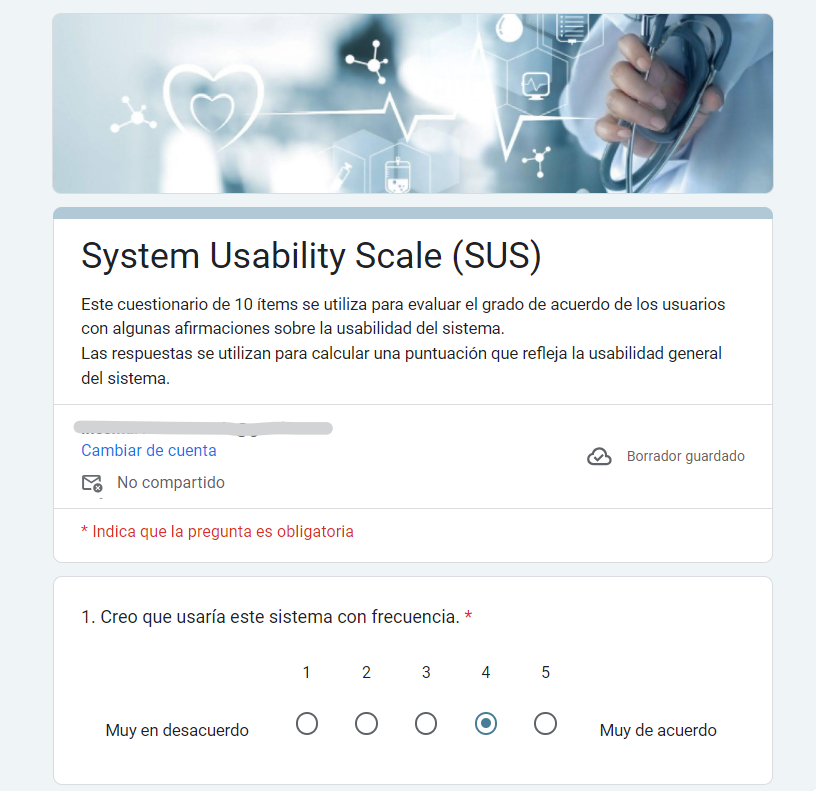
\includegraphics[width=1\textwidth]{img/G1_Resultados/sus1.png}
    \caption{Cuestionario SUS. Parte 1.}
    \label{fig:sus1}
\end{figure}

\begin{figure}[h]
    \centering
    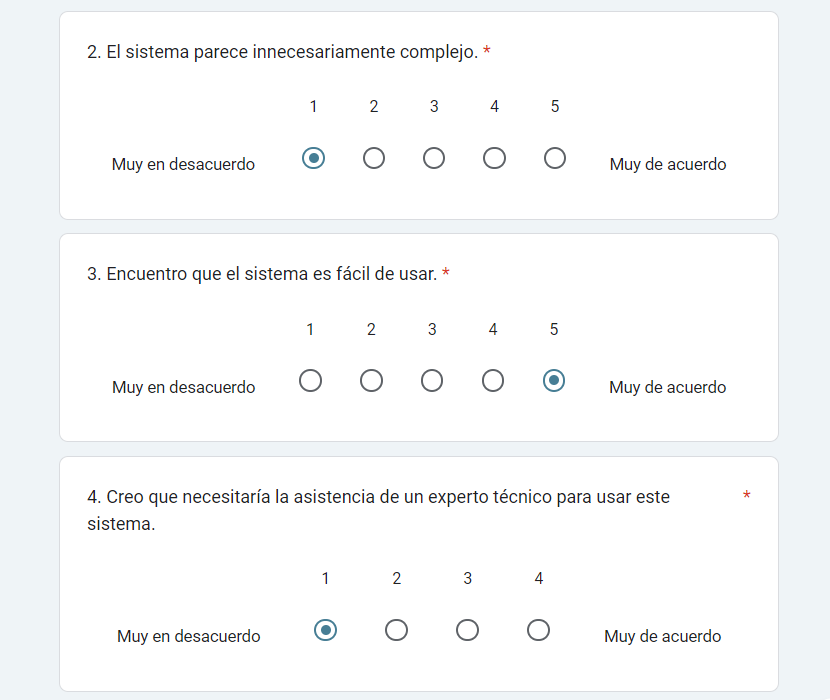
\includegraphics[width=1\textwidth]{img/G1_Resultados/sus2.png}
    \caption{Cuestionario SUS. Parte 2.}
    \label{fig:sus2}
\end{figure}

\begin{figure}[h]
    \centering
    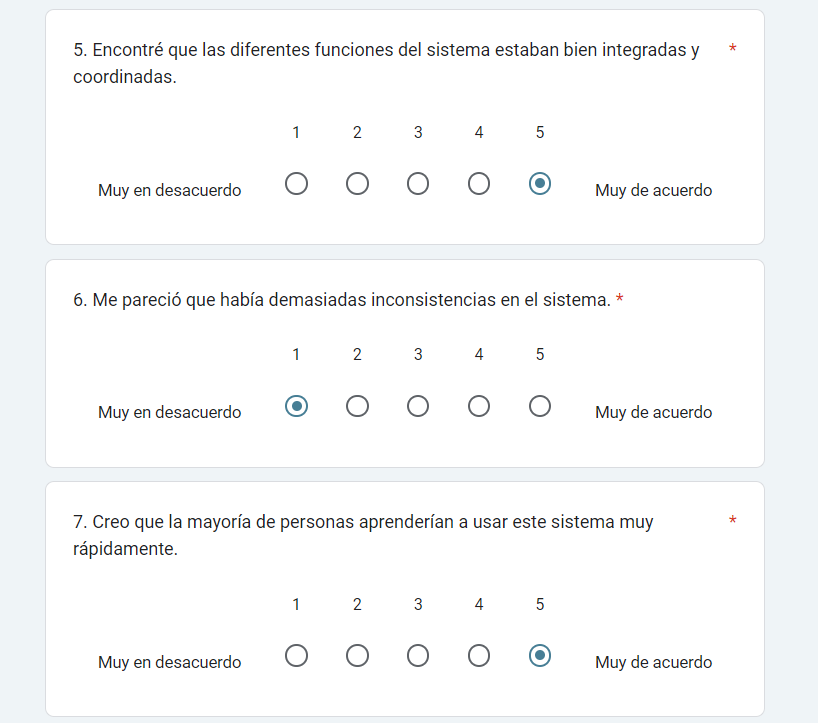
\includegraphics[width=1\textwidth]{img/G1_Resultados/sus3.png}
    \caption{Cuestionario SUS. Parte 3.}
    \label{fig:sus3}
\end{figure}

\begin{figure}[h]
    \centering
    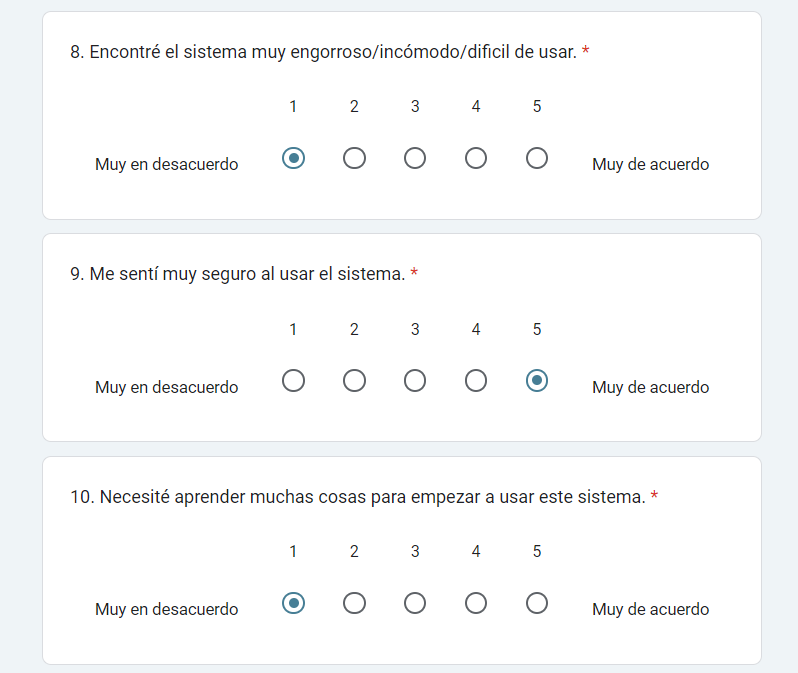
\includegraphics[width=1\textwidth]{img/G1_Resultados/sus4.png}
    \caption{Cuestionario SUS. Parte 4.}
    \label{fig:sus4}
\end{figure}

Para calcular la puntuación SUS, que pretende proporcionar un resultado objetivo sobre la usabilidad del sistema, se deben seguir los pasos descritos a continuación \cite{SUS}.
\begin{itemize}
    \item Suma de la puntuación de cada ítem (varía de 0 a 4) siguiendo las siguientes reglas para obtenerla:
    \begin{itemize}
        \item Ítems 1, 3, 5, 7 y 9, la puntuación es la posición en la escala menos 1.
        \item Ítems 2, 4, 6, 8 y 10, la puntuación es 5 menos la posición en la escala.
    \end{itemize}
    \item Multiplicar la suma de puntuaciones por 2.5.
\end{itemize}

En este caso se obtiene un \\SUS SCORE = ((3+4+4+4+4) + (4+4+4+4+4)) x 2.5 = 97.5 /100, \\resultado que supera ampliamente el punto de referencia (68) necesario para considerar que la web cumple de forma adecuada con su propósito.



